\chapter{Self-Consistent Fields}
\section{Massless Klein-Gordon Field with Dirichlet Boundary Conditions}

\begin{figure} \centering 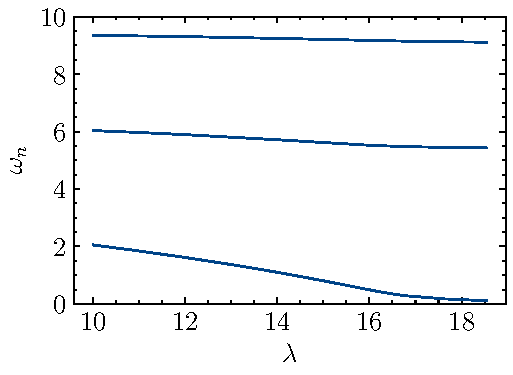
\includegraphics[width=0.5\linewidth]{figures/dirichlet/eigenvaluesHadamardDirichlet.pdf} \caption{Energy of the first three positive energy modes of the Klein-Gordon field as a function of the background electric field strength $\lambda$.} \label{fig:eigenvaluesHadamardDirichlet} \end{figure}

In this section, we present the results of the self-consistent solutions to the Klein-Gordon-Maxwell equations using the procedure outlined in the previous chapter. Figure \ref{fig:eigenvaluesHadamardDirichlet} shows the energy of the first three modes of the massless Klein-Gordon field as a function of the increasing background electric field strength $\lambda$. The lower curve corresponds to $\omega_1$, the middle curve to $\omega_2$ and the upper curve to $\omega_3$.
Notice that the energy of the first mode presents a very different high-$\lambda$ behavior from that seen in Figure \ref{fig:figures-eigenvalues-external-field-approximation-png}, which showed $\omega_1$ dropping sharply to 0 as $\lambda\to\lambda_c$.  In contrast, Figure \ref{fig:eigenvaluesHadamardDirichlet} shows how the back-reaction of the Klein-Gordon field effectively screens the background electric field, thereby raising the energy of the modes and preventing instabilities that would  otherwise arise in the external field approximation.

The negative energies are not shown in this plot since in the chosen gauge, $\omega_{-n} = -\omega_n$. 

\begin{figure} \begin{subfigure}{0.5\textwidth} \centering
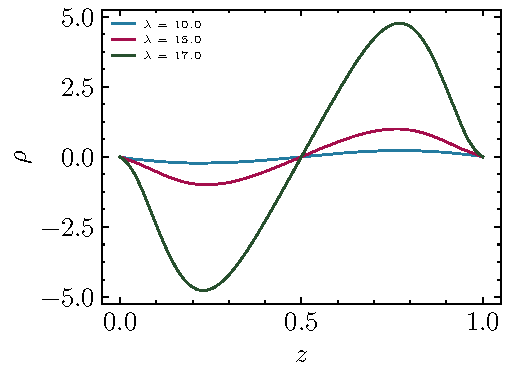
\includegraphics[width=1\linewidth]{figures/dirichlet/vacuumPolarizationEvolution.pdf}
\label{fig:HadamardVacuumPolarization1}
\end{subfigure}
\hfill
\begin{subfigure}{0.5\textwidth} 
\centering
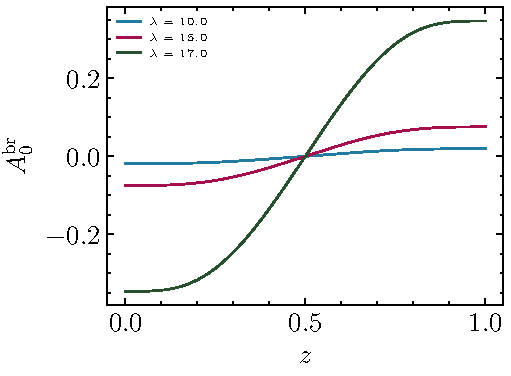
\includegraphics[width=1\linewidth]{figures/dirichlet/A0InducedEvolution.pdf} 
\label{fig:HadamardVacuumPolarization2} 
\end{subfigure}
\caption{Self-consistent vacuum polarization $\rho(z)$ (left) and their corresponding induced potential $A_0^\text{br}(z)$ (right) for select values of $\lambda$. } \label{fig:HadamardVacuumPolarization} \end{figure}

Figure \ref{fig:HadamardVacuumPolarization} illustrates both the self-consistent vacuum polarization $\rho(z)$ and the electrostatic potential $A_0^\text{br}(z) = -\int_{\frac{1}{2}}^z dz' \int_0^{z'}dz''{\rho}(z'')$ for selected values of $\lambda$. The back-reaction grows rapidly with $\lambda$ for higher values of $\lambda$. 
To better visualize the dependence of the vacuum polarization on $\lambda$, we study the induced charge due to the background electric field. The boundary conditions imposed in the equation \eqref{eq:poisson-br} imply that the induced charge $Q_{\text{total}}$
$$Q_{\text{total}} = \int_0^1 \rho(z) dz = 0.$$
It is easy to check that this holds since $\rho(z) = -\rho(1-z)$.
We instead focus on the induced charge in the left half of the $z$-region:
$$Q_{I} = \int_0^\frac{1}{2} \rho(z) dz.$$
In one spatial dimension, $Q_I$ coincides with the value of the induced electric field at $z=\frac{1}{2}$. We use this as a measure of the strength of the back-reaction. This charge causes the effective screening of the background electric field, and the measured electric field at $z=\frac{1}{2}$ is $Q_I + \lambda$. 

Figure \ref{fig:induced-charge} shows the induced charge $Q_I$  as a function of $\lambda$ (left panel), and the screened total charge $\lambda + Q_I$ observed at $z=\frac{1}{2}$ (right panel). The behavior of the induced charge $Q_I$ changes as $\lambda$ increases. For low $\lambda$ ($\lambda\lesssim10$), $Q_I$ decreases linearly with $\lambda$. As $\lambda$ approaches $\lambda_c$, we observe a rapid growth in the absolute value of $Q_I$,  screening the background electric field. The measured total electric field at $z=\frac{1}{2}$ never reaches $\lambda_c$, as is seen in the right pane of \ref{fig:induced-charge}.



 
%Figure \ref{fig:firstModeRho} illustrates the contributions of the modes $n=\pm1$ to the total charge density. In the top panel, the charge density $\rho_{1}$ associated to $n=1$, in the middle panel the charge density $\rho_{-1}$ associated to $n=-1$, and in the bottom panel their total contribution to the total charge density $\rho_1 + \rho_{-1}$. Notice how $\rho_1$ behaves as one would expect a positively charged particle to behave under a right-pointing electric field. Also notice how for a certain value of $\lambda$, a region of negative charge appears. Since $$\rho_n = (\omega_n + \lambda(z-1/2) - \epsilon A_0^\text{br}) \lvert\phi_n\rvert^2$$, this region corresponds to $$ $$

%\begin{figure}
%    \centering
%    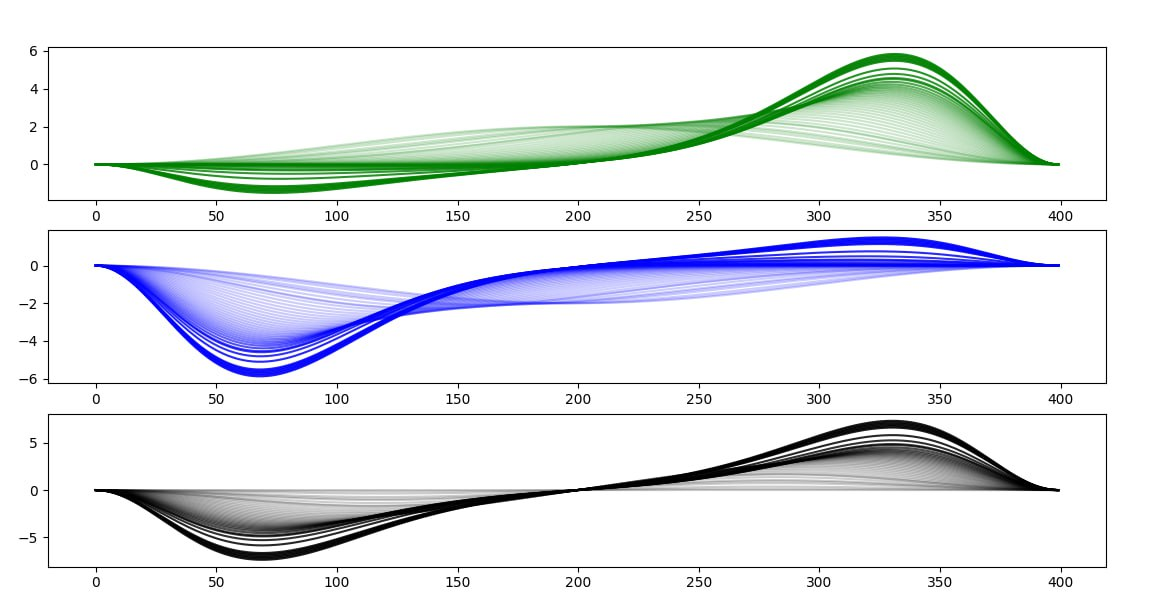
\includegraphics[width=0.75\linewidth]{figures/dirichlet/firstModeRho.jpg}
%    \caption{The charge density associated with the modes $n=1$ (top panel), $n=-1$ (middle panel) and their contribution to the total vacuum polarization $\rho_{1} + \rho_{-1}$ (bottom panel) for increasing $\lambda$ values, with dimmer curves corresponding to lower $\lambda$ values, and opaque curves corresponding to higher $\lambda$. }
%    \label{fig:firstModeRho}
%\end{figure}

\begin{figure}
\begin{subfigure}{0.5\textwidth}
    \centering
    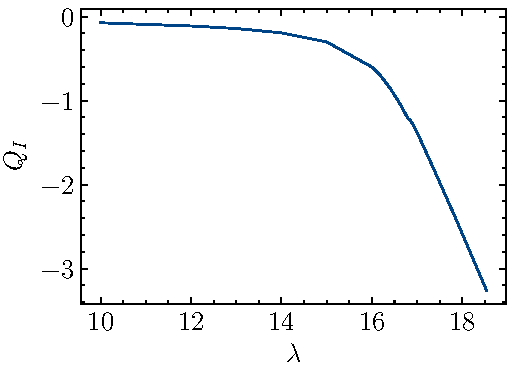
\includegraphics[width=0.95\linewidth]{figures/dirichlet/inducedCharge.pdf}
\end{subfigure}
\begin{subfigure}{0.5\textwidth}
    \centering
    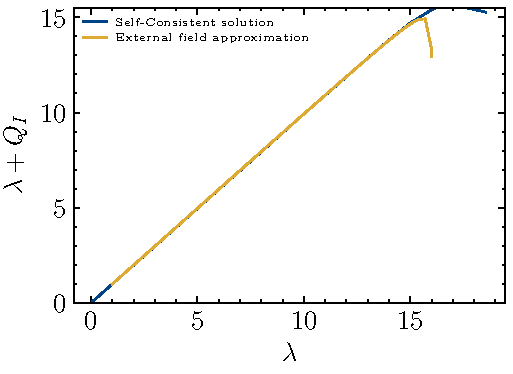
\includegraphics[width=0.95\linewidth]{figures/dirichlet/electricFieldInduced.pdf}
\end{subfigure}
\caption{The induced electric charge $Q_I = \int_0^{1/2}\rho(z)dz$ in the region $z\in[0,1/2]$ as a function of $\lambda$ (left pane) and the total electric field $\lambda + Q_I$ at the mid-point as a function of $\lambda$ (right pane).  }
\label{fig:induced-charge}
\end{figure}\subsection{In comparison with \cite{Ambj1983}}

\cite{Ambj1983} calculates the vacuum polarization without taking into account the parallel transport with respect to the gauge covariant derivative. Moreover, in the mode decomposition of the vacuum polarization only the first mode is considered. We have shown in Figure \ref{fig:perturbative-rho-comparison} the comparison between the perturbative incorrect non-inclusion of the parallel transport (blue) and with the inclusion thereof (orange). This figure illustrates a strong difference between these two recovered quantities. The left pane of Figure \ref{fig:lowLambdaVacuumPolarization} shows the comparison between the self-consistent vacuum polarizations, as calculated by including (orange) or not including (blue) the parallel transport in the renormalization procedure. For lower values of $\lambda$ the behavior of the self-consistent vacuum polarization is identical to the perturbative approximation, and therefore it is no surprise that for these values of $\lambda$ the self-consistent vacuum polarizations also present such big differences in behavior. 

However, as $\lambda$ increases and the system diverges from the perturbative behavior, the vacuum polarization calculated using Hadamard point-splitting rapidly "catches up" to the mode sum formula vacuum polarization. This explains how the correct renormalization procedure, although much weaker at lower values of $\lambda$, is also able to screen the background electric field as it increases.

\begin{figure}
\begin{subfigure}{0.5\textwidth}
    \centering
    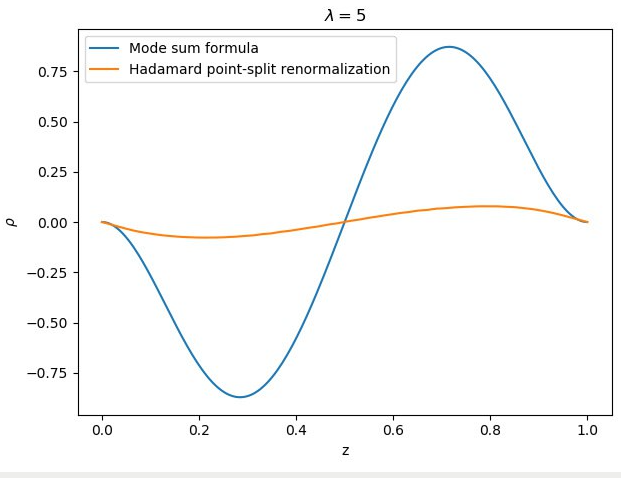
\includegraphics[width=0.75\linewidth]{figures/dirichlet/lowLambdaVacuumPolarizationComparison.png}
\end{subfigure}
\begin{subfigure}{0.5\textwidth}
    \centering
    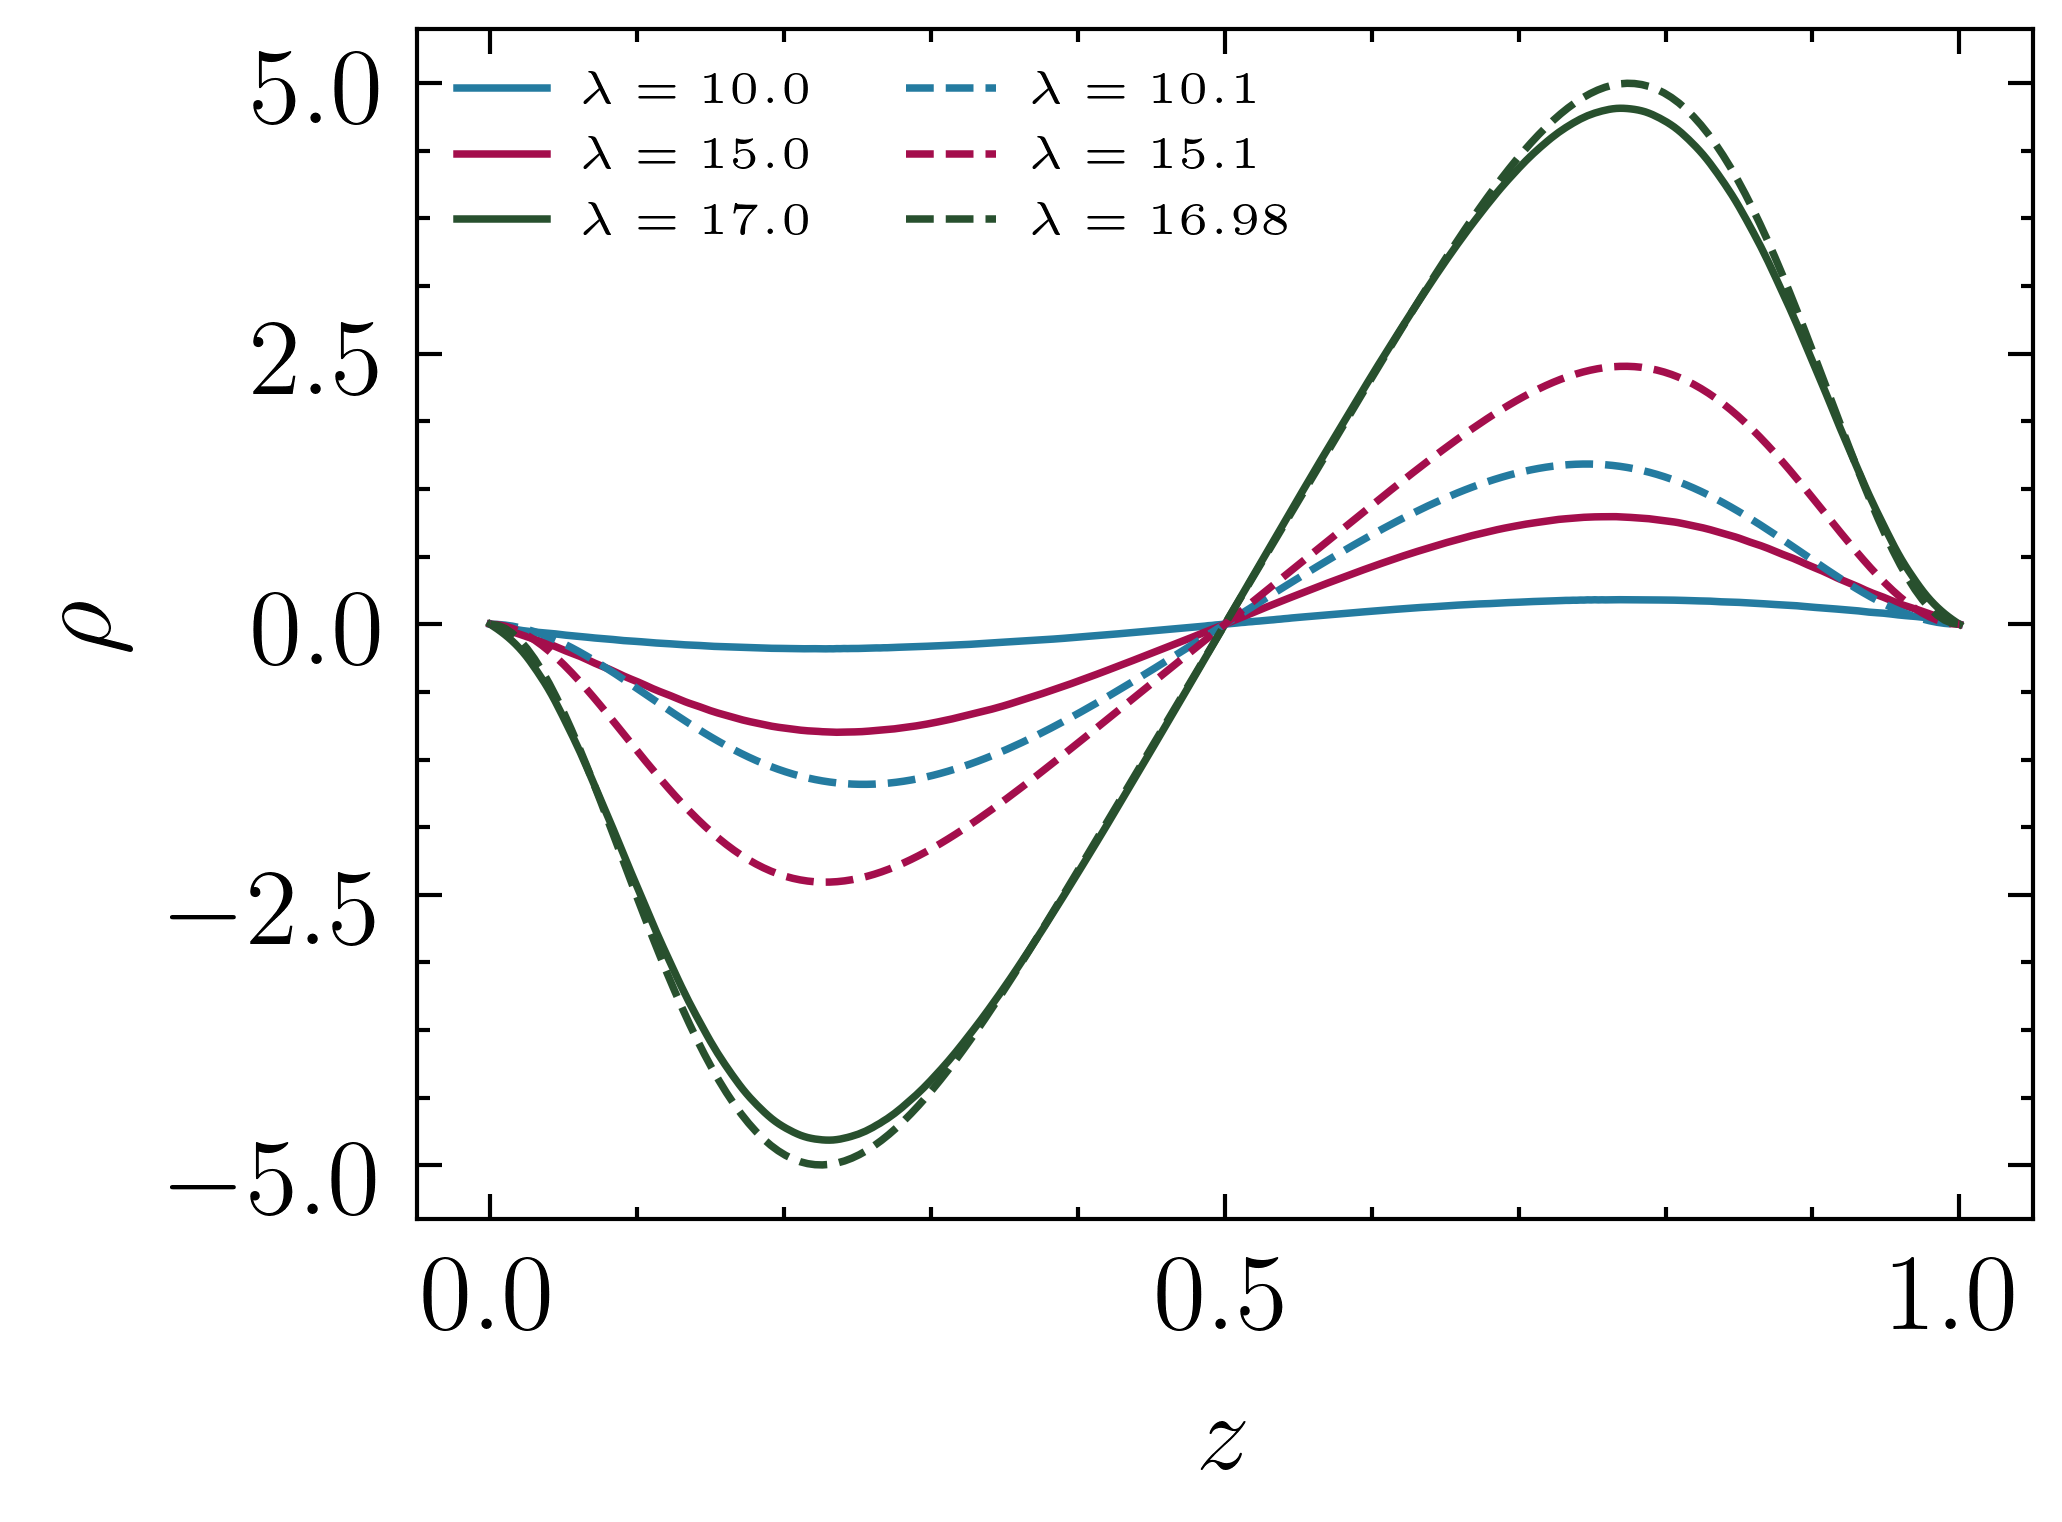
\includegraphics[width=0.75\linewidth]{figures/dirichlet/vacuumPolarizationEvolutionComparison.png} 
 \end{subfigure}
 \caption{Self-consistent vacuum polarizations for low $\lambda$ (left pane) as calculated using the (wrong) mode sum formula used in \cite{Ambj1983} in blue and the (correct) Hadamard point-splitting renormalization procedure described in the previous sections in orange. In the right pane, high $\lambda$ comparison of the self-consistent vacuum polarizations for $\lambda = 16, 17, 18.4$, beyond the critical $\lambda_c$. These comparisons need to be made in different plots due to the difference in scale of 2 orders of magnitude.}
    \label{fig:lowLambdaVacuumPolarization}
\end{figure}

Figure \ref{fig:different-lambda-rho} presents the induced charged $Q_I$ defined in the previous section for both renormalization schemes. This figure shows how the effective screening of the two methods are almost identical for higher values of $\lambda$.
\begin{figure}
    \centering
    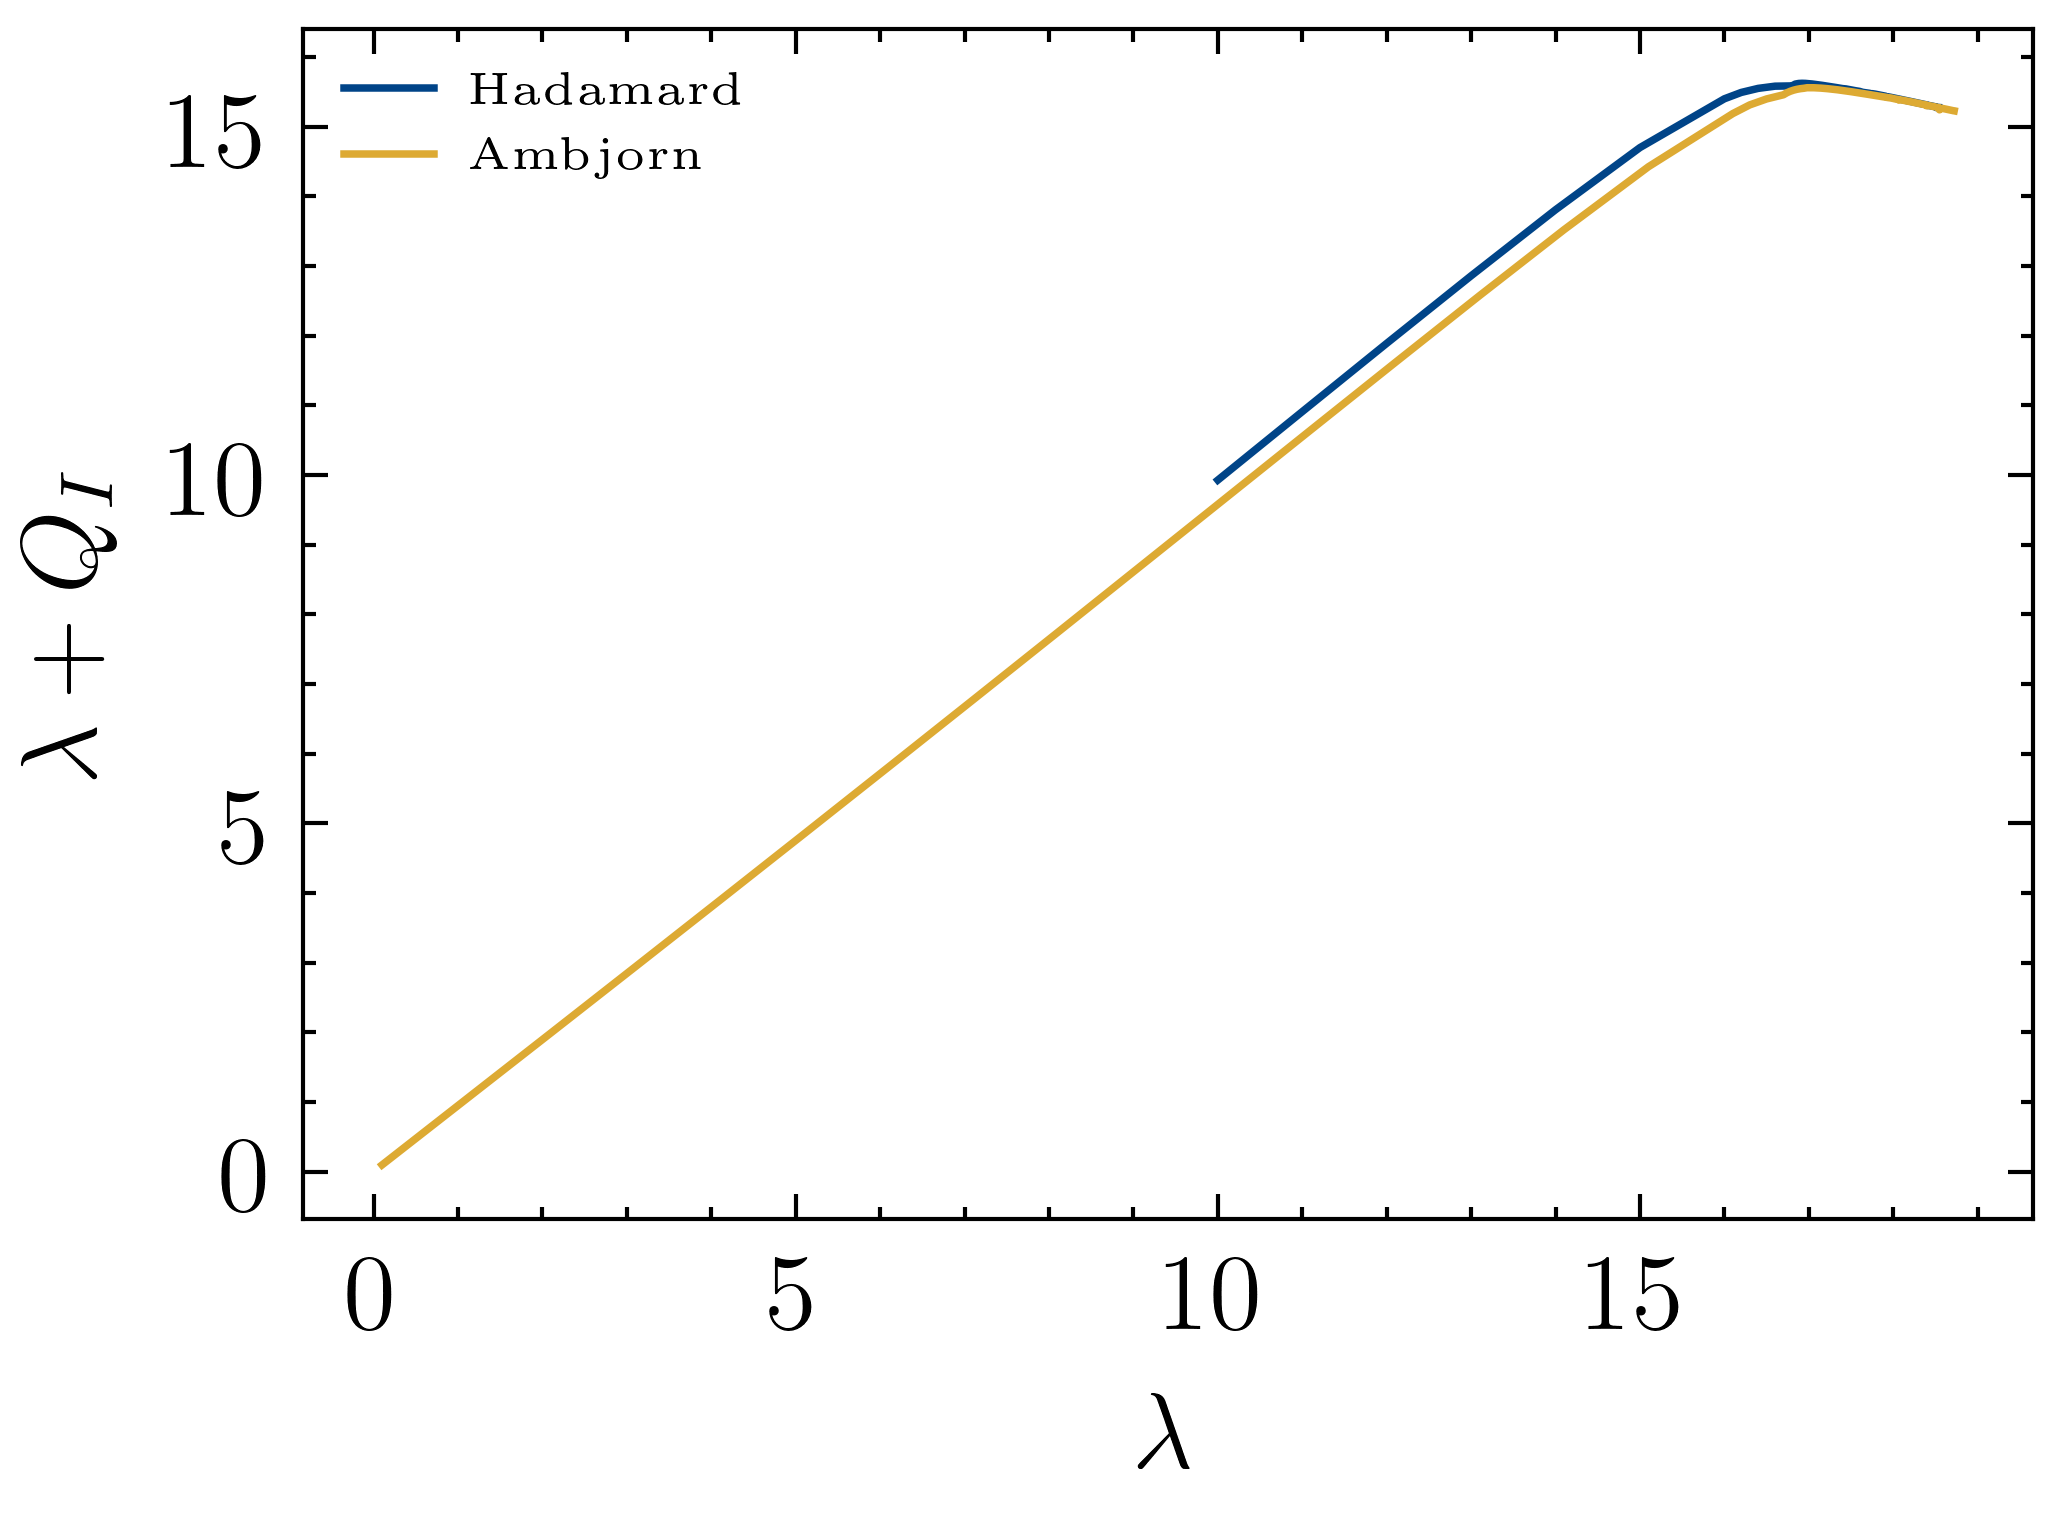
\includegraphics[width=0.5\linewidth]{figures/dirichlet/electricFieldInducedComparison.png}
    \caption{Comparison of the total electric field measured at $z=1/2$ for the two renormalization procedures. In blue, the electric field corresponding to the vacuum polarization as calculated by renormalization with respect to the Hadamard parametrix. In yellow, the resulting screening due to the vacuum polarization, when calculated using the mode sum formula as was used in \cite{Ambj1983}. Notice the perturbative region for $0 <\lambda \lesssim10$. For $\lambda \gtrsim 10$, the system can no longer be approximated to the perturbative case. } 
    \label{fig:different-lambda-rho}
\end{figure}

The induced electromagnetic potential $A_0^\text{br}$, being the second integral of the vacuum polarization presents the same behavior. 
\begin{figure}
    \centering
    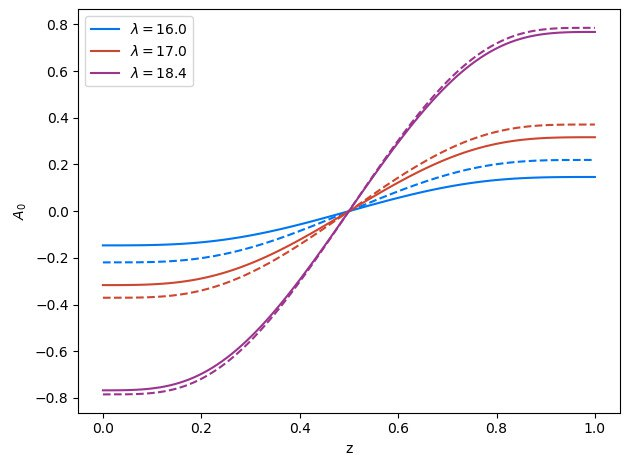
\includegraphics[width=0.5\linewidth]{figures/dirichlet/highLambdaValuesA0Induced.jpg}
    \caption{Comparison of the induced potentials $A_0^\text{br}$ using the same format as figure \ref{fig:highLambdaVacuumPolarization}.}
    \label{fig:enter-label}
\end{figure}

